\chapter{Constantes de equilíbrio e deslocamentos}\label{ch:b2:equilibrium-shifts}

Uma unidade de amônia opera seu conversor a cerca de \qty{450}{\celsius} e
\qty{200}{bar}. À temperatura ambiente, o equilíbrio \ce{N2 + 3H2 <=>
2NH3} está tão deslocado para o lado da amônia que uma mistura dos elementos
poderia, em princípio, ser convertida quase completamente; no entanto, os
engenheiros a aquecem, o que faz o equilíbrio recuar, e depois a comprimem
a duzentas atmosferas, o que custa muita energia. As razões são um
compromisso entre até onde uma reação pode ir e com que velocidade ela vai.
Este capítulo transforma a \omterm{def:b2:reaction-free-energy:gibbs-energy}{energia de Gibbs} dos capítulos anteriores na
constante de equilíbrio do volume do 1.º ano, mostra como essa constante
varia com a temperatura, conta quantas condições um experimentador pode
escolher livremente e prevê em que sentido um equilíbrio se desloca quando
se mudam a temperatura, a pressão ou a composição.

\begin{recall}
\Cref{ch:b2:reaction-free-energy}: o critério de evolução $\Delta_r G\,\dd\xi
\leq 0$ e a relação de Gibbs--Helmholtz;
\cref{ch:b2:chemical-potential}: $\Delta_r G = \Delta_r G^\circ + RT\ln Q$.
O volume do 1.º ano: o quociente $Q = \prod_i a_i^{\nu_i}$, a constante de
equilíbrio padrão $K^\circ$ como o valor de $Q$ no equilíbrio, a lei da
ação das massas e a regra ``$Q < K^\circ$: sentido direto'', todas
enunciadas ali como leis; as tabelas de avanço; os estados finais de uma ou
duas reações. Ele também prometeu que a escolha da temperatura e da pressão
para a amônia e para o trióxido de enxofre seria explicada aqui.
\end{recall}

\begin{omfigure}
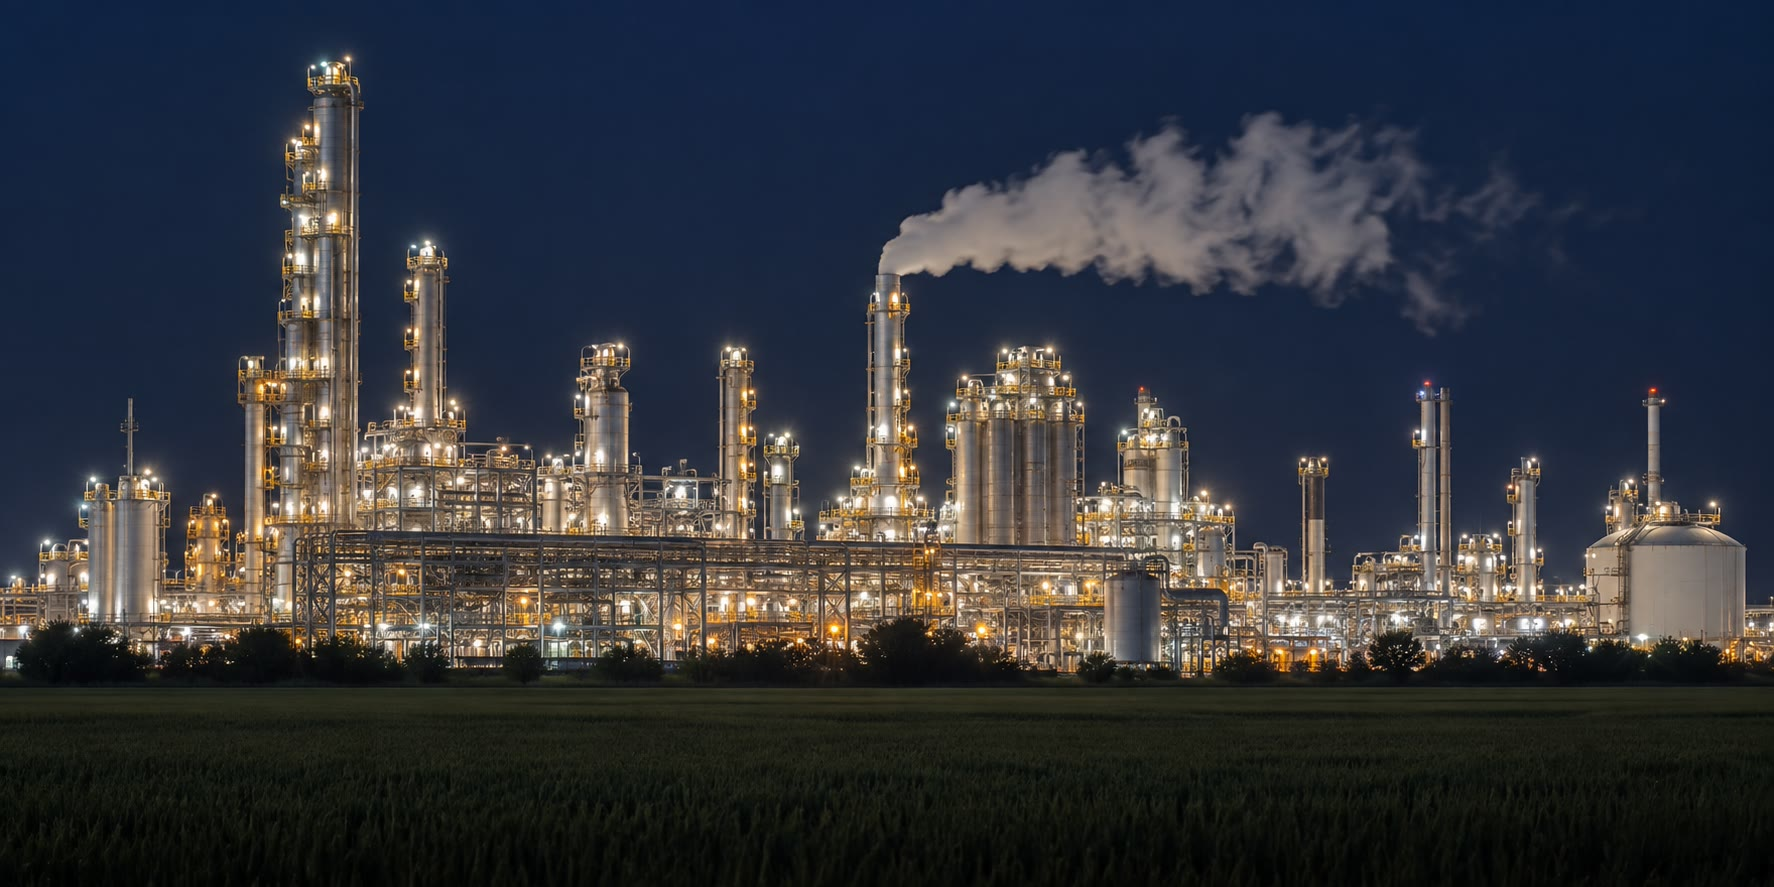
\includegraphics[width=0.7\linewidth]{images/book3/ai/b2-04-ammonia-plant.jpg}

{\small Uma unidade de amônia à noite. Em seu conversor, nitrogênio e
hidrogênio passam sobre um catalisador de ferro a algumas centenas de graus
e algumas centenas de bar; a escolha dessas condições é o assunto do
problema de fim de semana.}
\end{omfigure}

\section{A constante de equilíbrio a partir da energia de Gibbs}

\begin{theorem}[Constante de equilíbrio padrão]\label{thm:b2:equilibrium-shifts:k-from-g}
No equilíbrio, $\Delta_r G = 0$, e o quociente de reação assume o valor
\[
  K^\circ(T) = \exp\!\left(-\frac{\Delta_r G^\circ(T)}{RT}\right), \qquad
  \Delta_r G^\circ(T) = -RT\ln K^\circ(T) .
\]
Ela depende apenas da temperatura.
\end{theorem}

\begin{proof}
O critério de evolução faz de $\Delta_r G = 0$ a condição de equilíbrio.
Com $\Delta_r G = \Delta_r G^\circ + RT\ln Q$
(\cref{prop:b2:chemical-potential:delta-g-q}), o equilíbrio significa $\ln Q_{\text{eq}}
= -\Delta_r G^\circ/(RT)$, uma função apenas de $T$, já que $\Delta_r G^\circ$ o é.
\end{proof}

\begin{corollary}[As leis do volume do 1.º ano]\label{cor:b2:equilibrium-shifts:mass-action}
$\Delta_r G = RT\ln(Q/K^\circ)$. Logo, um sistema com $Q < K^\circ$ evolui
no sentido direto, um com $Q > K^\circ$ no sentido inverso, e um com $Q = K^\circ$
está em equilíbrio (a lei da ação das massas).
\end{corollary}

\begin{proof}
Substitua $\Delta_r G^\circ = -RT\ln K^\circ$ em $\Delta_r G = \Delta_r G^\circ
+ RT\ln Q$; o sinal de $\Delta_r G$ é o de $\ln(Q/K^\circ)$, e o
critério de evolução exige $\Delta_r G\,\dd\xi \leq 0$.
\end{proof}

\begin{example}[Três constantes a \qty{298}{K}]\label{ex:b2:equilibrium-shifts:constants}
Síntese da amônia, $\Delta_r G^\circ = \qty{-32.8}{kJ/mol}$: $K^\circ =
\exp(32\,800/(8.314 \times 298.15)) = \num{5.6e5}$ (as tabelas, com mais
algarismos, dão \num{5.4e5}). A dissociação do \ce{N2O4}, $\Delta_r G^\circ =
\qty{+4.7}{kJ/mol}$: $K^\circ = 0.15$. A decomposição do calcário,
$\Delta_r G^\circ = \qty{+130.4}{kJ/mol}$: $K^\circ = \num{1.5e-23}$, e a
pressão de equilíbrio do dióxido de carbono acima do calcário à temperatura
ambiente é de $\num{1.5e-23}$ bar, absolutamente nada. Uma variação de
\qty{5.7}{kJ/mol} em $\Delta_r G^\circ$ a \qty{298}{K} multiplica ou divide
$K^\circ$ por dez.
% ledger: dfh:NH3_g, s0:NH3_g, janafG:NH3.298.15 (computed in figdata/bachelor-2/thermo-data.py and vant-hoff.py)
\end{example}

A \omterm{def:b2:reaction-free-energy:gibbs-energy}{energia de Gibbs} do sistema inteiro mostra a mesma coisa como uma
paisagem: ela é mínima no avanço de equilíbrio, onde sua inclinação,
$\Delta_r G$, é nula.

\begin{omfigure}
\begin{tikzpicture}
\begin{axis}[
  width=0.7\linewidth, height=5.6cm, xmin=0, xmax=1, ymin=-2.2, ymax=5.2,
  axis x line=bottom, axis y line=left, xlabel={avanço $\xi$ (mol)},
  ylabel={$G(\xi) - G(0)$ (\unit{kJ})},
  tick label style={font=\small}, label style={font=\small}, clip=false]
\addplot[omDef, very thick] table[x=xi, y=G] {figdata/out/bachelor-2-gibbs-extent.dat};
\draw[dotted] (axis cs:0.189,-2.2) -- (axis cs:0.189,-0.949);
\fill[omThm] (axis cs:0.189,-0.949) circle (1.6pt);
\node[omThm, anchor=west, font=\small] at (axis cs:0.21,-1.75) {equilíbrio, $\xi = 0.189$};
\draw[dashed, gray] (axis cs:0,0) -- (axis cs:1,4.728);
\node[gray, font=\scriptsize, anchor=south east] at (axis cs:1,4.75) {$\xi\,\Delta_r G^\circ$};
\end{axis}
\end{tikzpicture}

{\small \omterm{def:b2:reaction-free-energy:gibbs-energy}{Energia de Gibbs} de um sistema fechado de gases perfeitos a
\qty{298}{K} e \qty{1}{bar}, partindo de \qty{1}{mol} de \ce{N2O4}, em
função do avanço de \ce{N2O4 <=> 2NO2}. Embora $\Delta_r G^\circ > 0$ (reta
tracejada, espécies puras), a mistura dos dois gases abaixa $G$, e o mínimo
fica em $\xi =
0.189$, onde $Q = K^\circ = 0.15$. À sua esquerda, a inclinação $\Delta_r G =
\partial G/\partial\xi$ é negativa; à sua direita, positiva.}
% ledger: dfh:N2O4_g, s0:N2O4_g, dfh:NO2_g, s0:NO2_g (computed in figdata/bachelor-2/gibbs-extent.py)
\end{omfigure}

\section{A temperatura: a equação de van 't Hoff}

\begin{theorem}[Equação de van 't Hoff]\label{thm:b2:equilibrium-shifts:vant-hoff}
\[
  \frac{\dd\ln K^\circ}{\dd T} = \frac{\Delta_r H^\circ(T)}{RT^2}
\]
(a \emph{equação de van 't Hoff}\index{equacao de van 't Hoff@equação de van 't Hoff}): a constante de
equilíbrio de uma reação \omterm{def:b2:reaction-enthalpy:exothermic}{endotérmica} aumenta com a temperatura, a de uma
reação \omterm{def:b2:reaction-enthalpy:exothermic}{exotérmica} diminui.
\end{theorem}

\begin{proof}
Escreva $\ln K^\circ = -\Delta_r G^\circ/(RT)$ e use a
\cref{prop:b2:reaction-free-energy:gibbs-helmholtz} (relação de Gibbs--Helmholtz),
\[
  \frac{\dd}{\dd T}\left(\frac{\Delta_r G^\circ}{T}\right) =
  -\frac{\Delta_r H^\circ}{T^2} ;
\]
divida por $-R$.
\end{proof}

\begin{proposition}[Forma integrada]\label{prop:b2:equilibrium-shifts:integrated}
Se $\Delta_r H^\circ$ é constante entre $T_1$ e $T_2$ (\omterm{def:b2:reaction-free-energy:ellingham-approximation}{aproximação de
Ellingham}),
\[
  \ln\frac{K^\circ(T_2)}{K^\circ(T_1)} = -\frac{\Delta_r H^\circ}{R}\left(
  \frac{1}{T_2} - \frac{1}{T_1}\right),
\]
e $\ln K^\circ$ é uma reta de inclinação $-\Delta_r H^\circ/R$ em função de
$1/T$.
\end{proposition}

\begin{proof}
Integre $\dd\ln K^\circ = (\Delta_r H^\circ/R)\,\dd T/T^2$, observando que
$\dd T/T^2 = -\dd(1/T)$.
\end{proof}

\begin{omfigure}
\begin{tikzpicture}
\begin{axis}[
  width=0.72\linewidth, height=5.8cm, xmin=0.9, xmax=3.5, ymin=-19, ymax=15,
  axis x line=bottom, axis y line=left, xlabel={$1000/T$ (\unit{1/K})},
  ylabel={$\ln K^\circ$}, tick label style={font=\small},
  label style={font=\small}, clip=false]
\addplot[omThm, dashed, thick] table[x=invT, y=lnK] {figdata/out/bachelor-2-vant-hoff-a-line.dat};
\addplot[omDef, only marks, mark=*, mark size=1.8pt] table[x=invT, y=lnK] {figdata/out/bachelor-2-vant-hoff-a.dat};
\node[omDef, font=\scriptsize, anchor=west] at (axis cs:3.36,13.2) {\qty{298}{K}};
\node[omDef, font=\scriptsize, anchor=north west] at (axis cs:1.03,-15.3) {\qty{1000}{K}};
\node[omThm, font=\small, anchor=south east, align=right] at (axis cs:2.4,8) {inclinação $-\Delta_r H^\circ(298)/R$\\ $= +11\,050$ K};
\end{axis}
\end{tikzpicture}

{\small A constante de \ce{N2 + 3H2 <=> 2NH3} segundo as tabelas (pontos,
de 298 a \qty{1000}{K}) e a reta de van 't Hoff traçada com $\Delta_r H^\circ$
a \qty{298}{K} (tracejada). A reação é \omterm{def:b2:reaction-enthalpy:exothermic}{exotérmica}: $K^\circ$ cai de
\num{5e5} para \num{3e-7}. A alta temperatura, os pontos ficam abaixo da
reta: $\Delta_r H^\circ$ fica mais negativa à medida que $T$ aumenta
(\cref{ex:b2:reaction-enthalpy:kirchhoff}).}
% ledger: janafG:NH3.298.15, janafG:NH3.400, janafG:NH3.500, janafG:NH3.600, janafG:NH3.700, janafG:NH3.800, janafG:NH3.900, janafG:NH3.1000, dfh:NH3_g (computed in figdata/bachelor-2/vant-hoff.py)
\end{omfigure}

\begin{method}[Uma constante de equilíbrio a outra temperatura]\label{met:b2:equilibrium-shifts:k-at-t}
\begin{enumerate}
  \item A partir das tabelas a \qty{298}{K}, calcule $\Delta_r H^\circ$, $\Delta_r
        S^\circ$ e $K^\circ(298)$.
  \item Use a \omterm{thm:b2:equilibrium-shifts:vant-hoff}{equação de van 't Hoff} integrada ou calcule
        $\Delta_r G^\circ(T) = \Delta_r H^\circ - T\Delta_r S^\circ$ e depois
        $K^\circ(T)$: as duas vias são a mesma aproximação.
  \item Para um intervalo amplo ou um $\Delta_r C_p^\circ$ grande, prefira os
        $\Delta_f G^\circ(T)$ tabelados; um erro de \qty{5.7}{kJ/mol} a \qty{298}{K}
        (ou de \qty{13}{kJ/mol} a \qty{700}{K}) é um fator dez em $K^\circ$.
\end{enumerate}
\end{method}

\begin{history}[Jacobus Henricus van 't Hoff]
\begin{minipage}[t]{0.2\linewidth}\vspace{0pt}
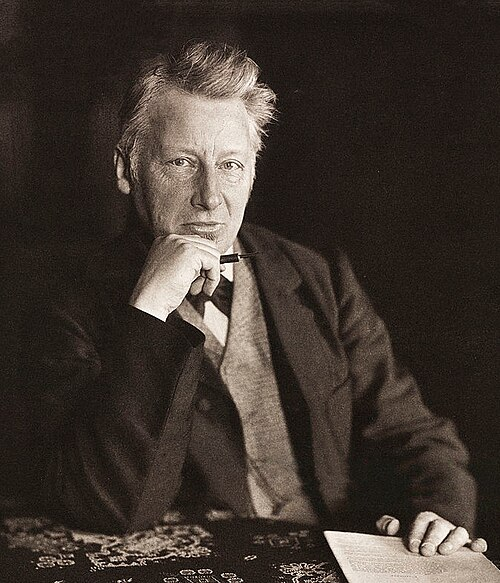
\includegraphics[width=\linewidth]{images/book3/vanthoff.jpg}
\end{minipage}\hfill
\begin{minipage}[t]{0.76\linewidth}\vspace{0pt}
Jacobus Henricus van 't Hoff (1852--1911) apresentou em 1884, em seus
\emph{Études de dynamique chimique}, a relação entre a temperatura e a
constante de equilíbrio que leva seu nome e, no ano seguinte, a lei da
\omterm{def:b2:chemical-potential:osmotic-pressure}{pressão osmótica} do \cref{ch:b2:chemical-potential}; dez anos antes, ele
havia proposto o átomo de carbono tetraédrico. Recebeu o primeiro Prêmio
Nobel de Química, em 1901. (Fotografia de N. Perscheid, 1904: domínio
público, Wikimedia Commons.)
\end{minipage}
\end{history}

\section{Variância}

Quantas grandezas intensivas um experimentador pode fixar livremente antes
que o estado de equilíbrio fique completamente determinado?

\begin{definition}[Variância]\label{def:b2:equilibrium-shifts:variance}
Os \emph{parâmetros intensivos independentes}\index{parametro intensivo independente@parâmetro intensivo independente}
de um sistema em equilíbrio são um conjunto de grandezas intensivas
(temperatura, pressão, frações molares em cada fase) que podem ser
escolhidas independentemente e que, uma vez escolhidas, fixam todas as
outras. Seu número é a
\emph{variância}\index{variancia@variância} $v$ do sistema.
\end{definition}

\begin{theorem}[Regra das fases]\label{thm:b2:equilibrium-shifts:phase-rule}
Para um sistema de $n$ espécies distribuídas entre $\varphi$ fases, ligadas por $r$
reações de equilíbrio independentes e por $s$ relações adicionais entre
grandezas intensivas fixadas pela preparação (uma alimentação
estequiométrica, a eletroneutralidade),
\[
  v = c + 2 - \varphi, \qquad c = n - r - s .
\]
\end{theorem}

\begin{proof}
Variáveis intensivas: $T$, $p$ e, em cada fase, as frações molares das
$n$ espécies, cuja soma é 1, ou seja, $n - 1$ livres por fase: ao todo $2 +
\varphi(n - 1)$. Relações: cada espécie está em equilíbrio entre as
fases, $\varphi - 1$ igualdades de \omterm{def:b2:chemical-potential:chemical-potential}{potenciais químicos} por espécie, $n(\varphi -
1)$ ao todo; cada reação dá $Q = K^\circ(T)$, $r$ relações; e $s$
relações adicionais. Subtraindo: $v = 2 + \varphi(n - 1) - n(\varphi - 1) - r -
s = n - r - s + 2 - \varphi$. (Uma espécie ausente de uma fase elimina, ao
mesmo tempo, uma variável e uma relação.)
\end{proof}

\begin{method}[Calcular uma variância]\label{met:b2:equilibrium-shifts:variance}
\begin{enumerate}
  \item Liste as espécies, com sua fase, e conte $n$ e $\varphi$
        (cada sólido puro é uma fase; todos os gases formam uma única fase).
  \item Conte as reações independentes $r$ entre elas.
  \item Conte as relações adicionais $s$: quantidades em proporção
        estequiométrica (somente se a relação é entre quantidades de uma
        mesma fase), eletroneutralidade de uma solução iônica.
  \item $v = n - r - s + 2 - \varphi$.
\end{enumerate}
\end{method}

\begin{example}[Três variâncias]\label{ex:b2:equilibrium-shifts:variances}
Calcário em um recipiente fechado, \ce{CaCO3(s) <=> CaO(s) + CO2(g)}: $n = 3$, $r =
1$, $\varphi = 3$ (dois sólidos, um gás): $v = 1$. Escolhida $T$, a pressão
do dióxido de carbono fica fixada: $p = K^\circ(T)\,p^\circ$. Uma mistura gasosa de
\ce{N2}, \ce{H2} e \ce{NH3} em equilíbrio: $n = 3$, $r = 1$, $\varphi = 1$, $v
= 3$ ($T$, $p$ e uma variável de composição); obtida a partir só da amônia, ou
de uma alimentação estequiométrica, \ce{N2} e \ce{H2} estão na razão 1 : 3, $s = 1$ e
$v = 2$: a $T$ e $p$ dados, a composição fica fixada, como usa o problema de
fim de semana.
\end{example}

\section{Deslocar um equilíbrio}

\begin{definition}[Deslocamento de um equilíbrio]\label{def:b2:equilibrium-shifts:shift}
Quando um sistema em equilíbrio é perturbado (uma variação de temperatura,
de pressão ou de uma quantidade), ele em geral deixa de estar em equilíbrio
e evolui para um novo equilíbrio. O \emph{deslocamento do equilíbrio}\index{deslocamento de um equilibrio@deslocamento de um equilíbrio}
ocorre no sentido direto se a reação avança ($\dd\xi > 0$) e no sentido
inverso caso contrário.
\end{definition}

\begin{method}[Prever um deslocamento]\label{met:b2:equilibrium-shifts:predict-shift}
Logo após a perturbação, calcule (ou estime o sinal da variação de)
$Q$ e $K^\circ$. Se agora $Q < K^\circ$, o deslocamento é no sentido direto; se $Q > K^\circ$,
no sentido inverso; se a igualdade continua valendo, não há deslocamento.
\end{method}

\begin{omfigure}
\begin{tikzpicture}[font=\small, >={Stealth}]
  \draw[->, thick] (0,0) -- (11,0) node[right] {$\ln Q$};
  \draw[omThm, thick] (5.5,0.25) -- (5.5,-0.25) node[below, align=center] {$\ln K^\circ$\\ ($= \ln Q$ antes)};
  \fill (5.5,0) circle (2pt);
  \draw[omDef, thick] (2.8,0.25) -- (2.8,-0.25) node[below] {$\ln Q$ logo após};
  \draw[->, omDef, very thick] (3.0,0.6) -- (5.2,0.6) node[midway, above] {sentido direto};
  \draw[omProp, thick] (8.4,0.25) -- (8.4,-0.25) node[below] {$\ln Q$ logo após};
  \draw[->, omProp, very thick] (8.2,0.6) -- (5.8,0.6) node[midway, above] {sentido inverso};
\end{tikzpicture}

{\small Uma perturbação move $Q$ (ou $K^\circ$, se a temperatura muda); o
sistema então se desloca até que de novo $Q = K^\circ$, no sentido direto se
$Q$ ficou pequeno demais, no inverso se ficou grande demais.}
\end{omfigure}

\begin{proposition}[Temperatura]\label{prop:b2:equilibrium-shifts:temperature}
A pressão constante, elevar a temperatura desloca um equilíbrio no sentido
\omterm{def:b2:reaction-enthalpy:exothermic}{endotérmico} (sentido direto se $\Delta_r H^\circ > 0$); abaixá-la, no
sentido \omterm{def:b2:reaction-enthalpy:exothermic}{exotérmico}.
\end{proposition}

\begin{proof}
A composição e pressão fixas, $Q$ não varia com $T$ (para sistemas
ideais); por van 't Hoff, $K^\circ$ aumenta com $T$ se $\Delta_r H^\circ >
0$. Logo após uma elevação de $T$, portanto, $Q < K^\circ$: sentido direto.
\end{proof}

\begin{proposition}[Pressão]\label{prop:b2:equilibrium-shifts:pressure}
A temperatura e composição constantes, elevar a pressão total de um
equilíbrio em fase gasosa o desloca no sentido que diminui o número de
moléculas de gás (sentido direto se $\Delta\nu_{\text{gás}} < 0$). Se $\Delta\nu_{\text{gás}}
= 0$, a pressão não tem efeito.
\end{proposition}

\begin{proof}
Com $p_i = x_ip$, $Q = \prod_i x_i^{\nu_i}\,(p/p^\circ)^{\Delta\nu_{\text{gás}}}$:
a composição fixa, elevar $p$ multiplica $Q$ por
$(p'/p)^{\Delta\nu_{\text{gás}}}$, que é $< 1$ se $\Delta\nu_{\text{gás}} <
0$. Então $Q < K^\circ$: sentido direto. As fases condensadas não contribuem.
\end{proof}

\begin{proposition}[Adição de um constituinte ou de um gás inerte]\label{prop:b2:equilibrium-shifts:adding}
Adicionar uma pequena quantidade de um constituinte gasoso $j$ a um equilíbrio
em fase gasosa muda $\ln Q$ de
\[
  \left(\frac{\partial\ln Q}{\partial n_j}\right) = \frac{\nu_j}{n_j} -
  \frac{\Delta\nu_{\text{gás}}}{n_{\text{tot}}}\ \ \text{mantidos constantes } T, p ;
  \qquad \frac{\nu_j}{n_j}\ \ \text{mantidos constantes } T, V .
\]
Adicionar um gás inerte não tem efeito a volume constante e, a pressão
constante, age como um abaixamento da pressão.
\end{proposition}

\begin{proof}
A $T$, $p$ constantes: $Q = \prod_i n_i^{\nu_i}\,(p/(p^\circ n_{\text{tot}}))^{
\Delta\nu_{\text{gás}}}$, cuja derivada logarítmica em relação a $n_j$ é
$\nu_j/n_j - \Delta\nu_{\text{gás}}/n_{\text{tot}}$ (primeiro termo nulo para
um gás inerte, $\nu_j = 0$). A $T$, $V$ constantes: $p_i = n_iRT/V$ e $Q = \prod_i n_i^{
\nu_i}\,(RT/(p^\circ V))^{\Delta\nu_{\text{gás}}}$, cuja derivada é apenas
$\nu_j/n_j$.
\end{proof}

\begin{remark}[Um reagente adicionado que faz a reação recuar]\label{rem:b2:equilibrium-shifts:paradox}
Na síntese da amônia, $\nu(\ce{N2}) = -1$ e $\Delta\nu_{\text{gás}} = -2$:
adicionar nitrogênio a $T$ e $p$ constantes muda $\ln Q$ de $-1/n_{\ce{N2}} +
2/n_{\text{tot}}$, que é positivo quando $x(\ce{N2}) > 1/2$. Em uma mistura
já rica em nitrogênio, adicionar mais nitrogênio dilui tanto o hidrogênio
que a amônia se decompõe. A regra ``adicionar um reagente desloca no sentido
direto'' é segura a volume constante, nem sempre a pressão constante.
\end{remark}

\begin{proposition}[Princípio de Le Chatelier]\label{prop:b2:equilibrium-shifts:le-chatelier}
As proposições acima se resumem no \emph{princípio de Le
Chatelier}\index{principio de Le Chatelier@princípio de Le Chatelier}: um sistema em equilíbrio,
perturbado em temperatura ou em pressão, se desloca no sentido que se opõe
à perturbação (absorve calor quando aquecido, reduz seu volume gasoso
quando comprimido).
\end{proposition}

\begin{proof}
Ele apenas reformula a \cref{prop:b2:equilibrium-shifts:temperature} (o sentido
\omterm{def:b2:reaction-enthalpy:exothermic}{endotérmico} absorve calor) e a \cref{prop:b2:equilibrium-shifts:pressure} (menos
moléculas de gás ocupam menos volume a mesmos $T$ e $p$). Para adições de
matéria a pressão constante, o princípio não é confiável
(\cref{rem:b2:equilibrium-shifts:paradox}): calcule $Q$.
\end{proof}

\begin{remark}[Quando o equilíbrio acaba]\label{rem:b2:equilibrium-shifts:rupture}
Um deslocamento pode terminar não em um novo equilíbrio, mas no
desaparecimento de uma fase. Aquecido em um recipiente fechado, o calcário
se decompõe até que $p(\ce{CO2}) =
K^\circ(T)\,p^\circ$; se não houver calcário suficiente para atingir essa
pressão, ele desaparece por completo e $Q$ fica abaixo de $K^\circ$: o sistema
fica definitivamente fora do equilíbrio, como o volume do 1.º ano já observara.
\end{remark}

\begin{history}[Henry Le Chatelier]
\begin{minipage}[t]{0.2\linewidth}\vspace{0pt}
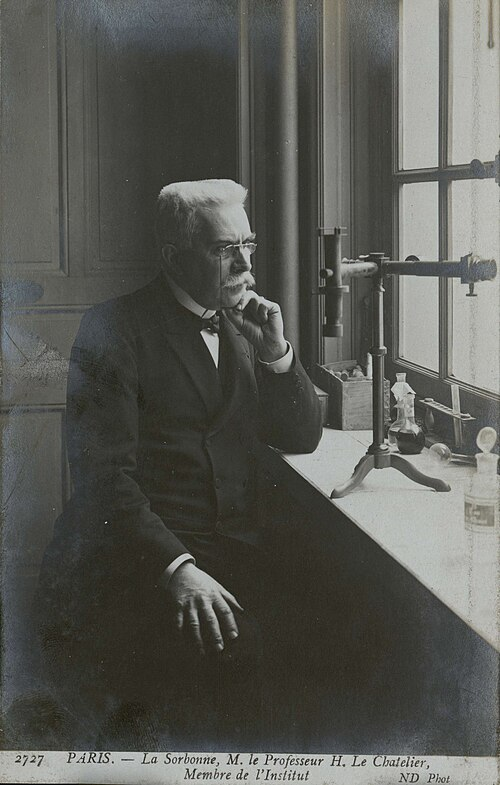
\includegraphics[width=\linewidth]{images/book3/lechatelier.jpg}
\end{minipage}\hfill
\begin{minipage}[t]{0.76\linewidth}\vspace{0pt}
Henry Le Chatelier (1850--1936), engenheiro de minas e químico que trabalhou
com cimentos, metalurgia e pirometria, enunciou em 1884 a ``lei de
\omterm{def:b2:equilibrium-shifts:shift}{deslocamento do equilíbrio}'' que leva seu nome. Ele também tentara, por
volta de 1901, produzir amônia a partir de seus elementos sob pressão; uma
explosão em seu aparelho pôs fim à tentativa. (Fotografia: autor
desconhecido, CC BY-SA 4.0, Wikimedia Commons.)
\end{minipage}
\end{history}

\section{Otimizar uma síntese}

\subsection*{A amônia}

\begin{omfigure}
\begin{tikzpicture}
\begin{axis}[
  width=0.78\linewidth, height=6.2cm, xmin=500, xmax=1000, ymin=0, ymax=0.9,
  axis x line=bottom, axis y line=left, xlabel={$T$ (K)},
  ylabel={fração molar de \ce{NH3} no equilíbrio},
  tick label style={font=\small}, label style={font=\small}, clip=false]
\addplot[omThm, very thick] table[x=T, y=p300] {figdata/out/bachelor-2-vant-hoff-b.dat};
\addplot[omDef, very thick] table[x=T, y=p200] {figdata/out/bachelor-2-vant-hoff-b.dat};
\addplot[omProp, very thick] table[x=T, y=p50] {figdata/out/bachelor-2-vant-hoff-b.dat};
\addplot[black!60, very thick] table[x=T, y=p1] {figdata/out/bachelor-2-vant-hoff-b.dat};
\node[omThm, font=\scriptsize, anchor=south west] at (axis cs:600,0.70) {300 bar};
\node[omDef, font=\scriptsize, anchor=north east] at (axis cs:612,0.52) {200 bar};
\node[omProp, font=\scriptsize, anchor=north east] at (axis cs:578,0.30) {50 bar};
\node[black!60, font=\scriptsize, anchor=south west] (onebar) at (axis cs:520,0.13) {1 bar};
\draw[black!60] (onebar.south west) -- (axis cs:512,0.075);
\draw[dotted] (axis cs:723,0) -- (axis cs:723,0.253);
\fill[omDef] (axis cs:723,0.253) circle (1.6pt);
\end{axis}
\end{tikzpicture}

{\small Fração molar de amônia no equilíbrio a partir de uma mistura 1 : 3 de
nitrogênio e hidrogênio (gases perfeitos), em função da temperatura, a quatro
pressões, calculada a partir das \omterm{def:b2:reaction-free-energy:gibbs-energy}{energias de Gibbs} tabeladas. A pressão a
eleva, a temperatura a abaixa; o ponto marca \qty{723}{K} e \qty{200}{bar}.}
% ledger: janafG:NH3.500, janafG:NH3.600, janafG:NH3.700, janafG:NH3.800, janafG:NH3.900, janafG:NH3.1000 (computed in figdata/bachelor-2/vant-hoff.py)
\end{omfigure}

A síntese é \omterm{def:b2:reaction-enthalpy:exothermic}{exotérmica} e reduz quatro moléculas de gás a duas: pelas
proposições acima, baixa temperatura e alta pressão favorecem a amônia.
A \qty{1}{bar} e à temperatura ambiente, o equilíbrio é quase total, mas
a reação simplesmente não ocorre: a ligação tripla do nitrogênio só se
rompe sobre um catalisador, e o catalisador de ferro só funciona a várias
centenas de graus. As unidades escolhem, portanto:
\begin{itemize}
  \item uma temperatura alta o bastante para a velocidade, tão baixa quanto o
        catalisador permite (cerca de \qty{700}{K});
  \item uma pressão alta para recuperar o rendimento perdido com a
        temperatura, limitada pelo custo da compressão e dos vasos de
        paredes espessas;
  \item um circuito: o gás que sai do conversor é resfriado, a amônia se
        condensa e é retirada, e o gás não convertido é reciclado com
        alimentação nova; uma pequena \omterm{def:b2:equilibrium-shifts:single-pass}{purga} elimina o argônio e o metano
        que, de outro modo, se acumulariam.
\end{itemize}

\begin{definition}[Conversão por passagem, reciclo, purga]\label{def:b2:equilibrium-shifts:single-pass}
Em um processo com reciclagem, a \emph{conversão por passagem}\index{conversao por passagem@conversão por passagem}
é a fração de um reagente convertida em uma passagem pelo
reator; a parte não convertida, separada do produto, volta à entrada do
reator como \emph{reciclo}\index{reciclo}; uma
\emph{purga}\index{purga} é uma pequena corrente retirada continuamente do
reciclo para impedir que espécies inertes se acumulem.
\end{definition}

\begin{omfigure}
\begin{tikzpicture}[font=\small, >={Stealth}, box/.style={draw, thick, rounded corners=2pt, minimum width=2.1cm, minimum height=1.0cm, align=center, fill=white}]
  \node[box] (comp) at (0,0) {compressor};
  \node[box] (conv) at (3.6,0) {conversor\\ (catalisador)};
  \node[box] (cond) at (7.2,0) {resfriador e\\ separador};
  \draw[->, thick] (-3.9,0) -- (comp) node[pos=0.0, above right] {\ce{N2 + 3H2} novo};
  \draw[->, thick] (comp) -- (conv);
  \draw[->, thick] (conv) -- (cond);
  \draw[->, thick, omDef] (cond.south) -- ++(0,-1.0) node[below] {amônia líquida};
  \draw[->, thick, omThm] (cond.north) -- ++(0,0.9) -| (comp.north);
  \node[omThm, above] at (2.6,1.4) {reciclo (gás não convertido)};
  \draw[->, thick, black!60] (6.1,1.4) -- (6.1,2.1) node[above] {purga};
\end{tikzpicture}

{\small O circuito da amônia. Cada passagem converte apenas parte do gás; a
amônia é retirada por condensação, e o restante é recomprimido e enviado de
volta com a alimentação nova. A \omterm{def:b2:equilibrium-shifts:single-pass}{purga} impede o acúmulo do argônio e do
metano, que não reagem.}
\end{omfigure}

\begin{history}[Haber e Bosch]
\begin{minipage}[t]{0.15\linewidth}\vspace{0pt}
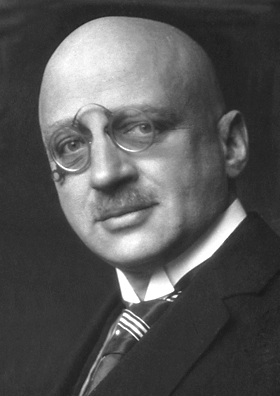
\includegraphics[width=\linewidth]{images/book3/haber.png}
\end{minipage}\hspace{0.01\linewidth}%
\begin{minipage}[t]{0.15\linewidth}\vspace{0pt}
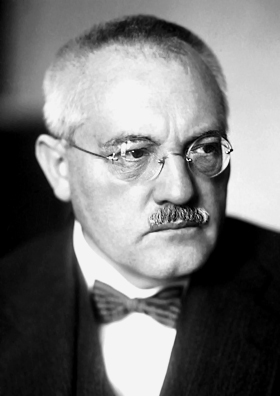
\includegraphics[width=\linewidth]{images/book3/bosch.jpg}
\end{minipage}\hfill
\begin{minipage}[t]{0.66\linewidth}\vspace{0pt}
Fritz Haber (1868--1934) mediu o equilíbrio da amônia sob pressão e, em
1909, a fez fluir continuamente de um conversor de laboratório sobre um
catalisador de ósmio. Carl Bosch (1874--1940) transformou isso em uma
indústria, com vasos de aço que resistiam ao hidrogênio quente sob pressão
e um catalisador de ferro barato; a primeira unidade entrou em operação em
1913. Haber recebeu o Prêmio Nobel em 1918, Bosch em 1931. (Retratos da
Fundação Nobel: domínio público, Wikimedia Commons.)
\end{minipage}
\end{history}

\subsection*{O trióxido de enxofre}

No processo de contato, \ce{2SO2(g) + O2(g) <=> 2SO3(g)} ($\Delta_r H^\circ =
\qty{-197.8}{kJ/mol}$ para a equação tal como está escrita) ocorre sobre um
catalisador de óxido de vanádio, ativo apenas a quente, em vários leitos
adiabáticos. Em cada leito, o calor liberado eleva a temperatura, o que
diminui $K^\circ$; a conversão para quando o gás atinge a curva de
equilíbrio. O resfriamento entre os leitos o traz de volta a uma
temperatura em que o equilíbrio permite mais conversão.
% ledger: dfh:SO2_g, dfh:SO3_g

\begin{omfigure}
\begin{tikzpicture}
\begin{axis}[
  width=0.72\linewidth, height=6.4cm, xmin=600, xmax=900, ymin=0, ymax=1.08,
  axis x line=bottom, axis y line=left, xlabel={$T$ (K)},
  ylabel={conversão do \ce{SO2}}, tick label style={font=\small},
  label style={font=\small}, clip=false]
\addplot[black, very thick] table[x=T, y=X] {figdata/out/bachelor-2-vant-hoff-c.dat};
\addplot[omThm, thick] table[x=T, y=X] {figdata/out/bachelor-2-vant-hoff-bed1.dat};
\addplot[omThm, thick] table[x=T, y=X] {figdata/out/bachelor-2-vant-hoff-bed2.dat};
\addplot[omThm, thick] table[x=T, y=X] {figdata/out/bachelor-2-vant-hoff-bed3.dat};
\draw[->, omDef, thick] (axis cs:892.8,0.676) -- (axis cs:712,0.676);
\draw[->, omDef, thick] (axis cs:784.4,0.924) -- (axis cs:712,0.924);
\node[font=\scriptsize, anchor=south west] at (axis cs:860,0.84) {equilíbrio};
\node[omThm, font=\scriptsize, anchor=west] at (axis cs:800,0.24) {leito 1 (adiabático)};
\node[omDef, font=\scriptsize, anchor=south] at (axis cs:800,0.68) {resfriamento};
\end{axis}
\end{tikzpicture}

{\small Conversão de equilíbrio de \ce{SO2} em \ce{SO3} em função da
temperatura (em preto) para uma alimentação modelo com \qty{10}{\percent}
de \ce{SO2} e \qty{11}{\percent} de \ce{O2} a \qty{1}{bar}, e o caminho do
gás através de três leitos adiabáticos (em vermelho, subindo em temperatura
à medida que a reação aquece o gás), resfriado entre os leitos (em azul).}
% ledger: janafG:SO2.600, janafG:SO2.700, janafG:SO2.800, janafG:SO2.900, janafG:SO3.600, janafG:SO3.700, janafG:SO3.800, janafG:SO3.900 (computed in figdata/bachelor-2/vant-hoff.py; feed and adiabatic rise are model values)
\end{omfigure}

\section{Exercícios}

\begin{exercise}[$\star$]\label{exo:b2:equilibrium-shifts:1}
Calcule $K^\circ$ a \qty{298}{K} para uma reação com $\Delta_r G^\circ =
\qty{-32.8}{kJ/mol}$, depois para $\Delta_r G^\circ = \qty{+32.8}{kJ/mol}$.
Que variação de $\Delta_r G^\circ$ multiplica $K^\circ$ por 100?
\end{exercise}

\begin{exercise}[$\star$]\label{exo:b2:equilibrium-shifts:2}
Para a síntese da amônia, $K^\circ(298) = \num{5.4e5}$ e $\Delta_r H^\circ =
\qty{-91.9}{kJ/mol}$. Estime $K^\circ$ a \qty{400}{K} com a \omterm{thm:b2:equilibrium-shifts:vant-hoff}{equação de van 't
Hoff} integrada; as tabelas dão 35.6.
\end{exercise}

\begin{exercise}[$\star$]\label{exo:b2:equilibrium-shifts:3}
Calcule a \omterm{def:b2:equilibrium-shifts:variance}{variância} de: (a) água líquida em equilíbrio com seu vapor;
(b) \ce{CaCO3(s) <=> CaO(s) + CO2(g)} em um recipiente fechado; (c) \ce{N2},
\ce{H2}, \ce{NH3} em equilíbrio, alimentação qualquer; (d) \ce{C(s) + H2O(g) <=>
CO(g) + H2(g)}.
\end{exercise}

\begin{exercise}[$\star$]\label{exo:b2:equilibrium-shifts:4}
Para \ce{N2O4(g) <=> 2NO2(g)}, $\Delta_r H^\circ > 0$. Em que sentido o
equilíbrio é deslocado por um aquecimento a pressão constante, por uma
compressão a temperatura constante, por uma adição de argônio a volume constante?
\end{exercise}

\begin{exercise}[$\star\star$]\label{exo:b2:equilibrium-shifts:5}
Para \ce{N2(g) + O2(g) <=> 2NO(g)}, $\Delta_r H^\circ = \qty{180.6}{kJ/mol}$,
$\Delta_r S^\circ = \qty{24.8}{J/(K.mol)}$. Calcule $K^\circ$ a \qty{298}{K}
e a \qty{2000}{K} (\omterm{def:b2:reaction-free-energy:ellingham-approximation}{aproximação de Ellingham}) e a fração molar de
\ce{NO} no ar ($x(\ce{N2}) = 0.78$, $x(\ce{O2}) = 0.21$, pouco consumidos) no
equilíbrio a \qty{2000}{K}. Por que os motores produzem esse poluente, e por que
ele sobrevive no escapamento resfriado?
\end{exercise}

\begin{exercise}[$\star\star$]\label{exo:b2:equilibrium-shifts:6}
Uma esterificação $\mathrm{A + B \rightleftharpoons E + W}$ em fase líquida
tem $K^\circ = 4.0$ (atividades tomadas como frações molares). Partindo de
\qty{1.0}{mol} de ácido A, calcule a quantidade de éster com \qty{1.0}{mol} e depois com
\qty{3.0}{mol} de álcool B. Explique, com $Q$ e $K^\circ$, por que retirar a
água à medida que ela se forma leva a reação até o fim.
\end{exercise}

\begin{exercise}[$\star\star$]\label{exo:b2:equilibrium-shifts:7}
A \qty{298}{K} e \qty{1}{bar}, $K^\circ = 0.148$ para \ce{N2O4 <=> 2NO2}.
Calcule o grau de dissociação de \qty{1}{mol} de \ce{N2O4}. Em seguida,
adiciona-se \qty{1}{mol} de argônio a pressão total constante: calcule o novo
grau de dissociação e explique. O que acontece se o argônio for adicionado a
volume constante?
\end{exercise}

\begin{exercise}[$\star\star$]\label{exo:b2:equilibrium-shifts:8}
O cloreto de amônio sublima dissociando-se, \ce{NH4Cl(s) <=> NH3(g) +
HCl(g)}. Calcule a \omterm{def:b2:equilibrium-shifts:variance}{variância} quando o gás é formado apenas pelo sólido e
quando se adicionou um pouco de amônia. O que cada caso significa para o
experimentador?
\end{exercise}

\begin{exercise}[$\star\star$]\label{exo:b2:equilibrium-shifts:9}
As tabelas dão, para a síntese da amônia, $K^\circ = 0.0993$ a \qty{500}{K} e
$K^\circ = \num{1.72e-3}$ a \qty{600}{K}. Deduza $\Delta_r H^\circ$ nesse
intervalo e compare com seu valor a \qty{298}{K}.
\end{exercise}

\begin{exercise}[$\star\star\star$]\label{exo:b2:equilibrium-shifts:10}
Demonstre o contraexemplo da \cref{rem:b2:equilibrium-shifts:paradox}: escreva
o $Q$ da síntese da amônia com as quantidades e a pressão total, calcule
$\partial\ln Q/\partial n(\ce{N2})$ a $T$ e $p$ constantes, e encontre a
condição sobre $x(\ce{N2})$ para a qual adicionar nitrogênio desloca o
equilíbrio no sentido inverso. O mesmo pode acontecer a volume constante?
\end{exercise}

\begin{exercise}[$\star\star\star$]\label{exo:b2:equilibrium-shifts:11}
O calcário é aquecido a \qty{1100}{K} em um recipiente fechado e vazio de
\qty{10.0}{L}, onde $\Delta_r G^\circ = \qty{1.62}{kJ/mol}$ para sua
decomposição (\cref{ch:b2:reaction-free-energy}). Calcule $K^\circ$ e a
pressão de equilíbrio do dióxido de carbono. Encontre o estado final para
\qty{0.050}{mol} e para \qty{0.200}{mol} de calcário.
\end{exercise}

\begin{exercise}[$\star\star\star$]\label{exo:b2:equilibrium-shifts:12}
Leia, na figura do processo de contato, a conversão e a temperatura na
saída de cada leito. Explique por que um único leito adiabático, por mais
longo que seja, não poderia ultrapassar cerca de 68\,\% de conversão com
essa alimentação, por que o gás é resfriado entre os leitos em vez de se
manter o catalisador frio o tempo todo, e o que limita a conversão do
último leito.
\end{exercise}

\section{Problema: O circuito da amônia}

\begin{problem}[{Problema de fim de semana --- a constante de equilíbrio da
síntese da amônia e sua dependência com a temperatura, a composição nas
condições do conversor, os deslocamentos causados pela pressão, pela
temperatura e pelos gases inertes, e o circuito}]
\label{pb:b2:equilibrium-shifts:1}
A amônia é produzida por \ce{N2(g) + 3H2(g) <=> 2NH3(g)} a partir de uma
alimentação estequiométrica.
Dados: a \qty{298.15}{K}, $\Delta_f H^\circ(\ce{NH3}) = \qty{-45.94}{kJ/mol}$,
$S^\circ_m$ (\unit{J/(K.mol)}) \ce{NH3} 192.77, \ce{N2} 191.61, \ce{H2} 130.68;
as tabelas dão $\Delta_f G^\circ(\ce{NH3}) = \qty{+27.19}{kJ/mol}$ a
\qty{700}{K} e \qty{+38.66}{kJ/mol} a \qty{800}{K}. Os gases são perfeitos;
$R = \qty{8.314}{J/(K.mol)}$.
% ledger: dfh:NH3_g, s0:NH3_g, s0:N2_g, s0:H2_g, janafG:NH3.700, janafG:NH3.800

\medskip
\noindent\textbf{Parte I --- A constante.}
\begin{enumerate}
  \item Calcule $\Delta_r H^\circ$, $\Delta_r S^\circ$ e $\Delta_r G^\circ$ a
        \qty{298}{K}, e $K^\circ(298)$.
  \item Calcule $K^\circ$ a \qty{700}{K} e a \qty{800}{K} a partir das tabelas.
  \item Deduza desses dois valores o $\Delta_r H^\circ$ médio entre
        \qty{700}{K} e \qty{800}{K} e compare com a questão 1.
  \item Estime $K^\circ(\qty{723}{K})$ a partir dos dois valores tabelados com
        a \omterm{thm:b2:equilibrium-shifts:vant-hoff}{equação de van 't Hoff}.
  \item Calcule $K^\circ(\qty{723}{K})$ na \omterm{def:b2:reaction-free-energy:ellingham-approximation}{aproximação de Ellingham} a partir
        dos dados a \qty{298}{K} e comente a diferença.
\end{enumerate}

\medskip
\noindent\textbf{Parte II --- O equilíbrio no conversor.}
\begin{enumerate}[resume]
  \item A partir de uma alimentação de \qty{1}{mol} de \ce{N2} e \qty{3}{mol} de \ce{H2}, escreva as
        quantidades no avanço $\xi$ e a quantidade total.
  \item Mostre que, sendo $x$ a fração molar da amônia, as frações molares
        de \ce{N2} e \ce{H2} são $(1-x)/4$ e $3(1-x)/4$.
  \item Mostre que $\dfrac{x}{(1-x)^2} = \dfrac{\sqrt{27}}{16}\,\dfrac{p}{p^\circ}\,
        \sqrt{K^\circ}$.
  \item Calcule $x$ a \qty{723}{K} e \qty{1}{bar}.
  \item Calcule $x$ a \qty{723}{K} e \qty{200}{bar}.
  \item Calcule a \omterm{def:b2:equilibrium-shifts:variance}{variância} do sistema e explique por que $T$ e $p$ fixam a
        composição.
\end{enumerate}

\medskip
\noindent\textbf{Parte III --- Os deslocamentos.}
\begin{enumerate}[resume]
  \item Sem calcular, em que sentido o equilíbrio se desloca quando a pressão
        aumenta? E quando a temperatura aumenta?
  \item O argônio entra com o ar usado para obter o nitrogênio. A pressão
        total constante, como sua presença desloca o equilíbrio?
  \item Uma mistura em equilíbrio tem $x(\ce{N2}) = 0.30$. Adicionar um pouco
        de nitrogênio a $T$ e $p$ constantes a desloca no sentido direto ou no inverso?
  \item A resposta mudaria a volume constante?
  \item Antes que o gás volte ao conversor, sua amônia é retirada por
        condensação. O que isso faz com $Q$ na entrada do conversor?
\end{enumerate}

\medskip
\noindent\textbf{Parte IV --- O circuito.}
\begin{enumerate}[resume]
  \item O gás sai do conversor com \qty{18}{\percent} de amônia, abaixo do
        valor de equilíbrio. Por que um conversor real não atinge o
        equilíbrio?
  \item Calcule a \omterm{def:b2:equilibrium-shifts:single-pass}{conversão por passagem} do hidrogênio correspondente a
        $x(\ce{NH3}) = 0.18$ a partir de uma alimentação estequiométrica.
  \item O gás não convertido é reciclado. Em regime estacionário, \qty{1.00}{mol}
        de \ce{N2} novo entra por unidade de tempo: quanta amônia sai, e quanto
        nitrogênio passa pelo conversor por unidade de tempo?
  \item Por que é preciso purgar um pouco de gás do \omterm{def:b2:equilibrium-shifts:single-pass}{reciclo}?
  \item Por que o conversor não opera a \qty{500}{K}, onde o equilíbrio é
        muito mais favorável?
  \item Dê a fração molar de amônia no equilíbrio a \qty{723}{K} e
        \qty{200}{bar} para uma alimentação estequiométrica, no modelo dos
        gases perfeitos.
\end{enumerate}
\end{problem}
